\begin{definition}[Imersão]
  Sejam $U\subseteq\mathbb{R}^{m}$ e $f:U\to\mathbb{R}^{n}$ diferenciável. Dizemos que $f$ é uma \textbf{imersão} no ponto $a\in U$ se a derivada $f^{\prime}(a):\mathbb{R}^{m}\to\mathbb{R}^{n}$ é uma transformação linear injetiva.\\
  Se $f$ é uma imersão em todos os pontos de $U$, dizemos que $f$ é uma imersão.\\
  Se $f^{\prime}(a)$ é injetiva e $f^{\prime}$ é contínua em $a$, então existe uma vizinhança de $a$ que transforma uma bola centrada em $a$, homeomorficamente sobre sua imagen ($|f(x)-f(y)|\geq c|x-y|$). 
\end{definition}
\begin{note}
  Note que a composta de duas imersões é uma imersão.
\end{note}
\begin{example}
  Seja $f:\mathbb{R}^{m}\to\mathbb{R}^{m} \times\mathbb{R}^{m}$ dada por $f(x)=(x,0)$. Logo como $f$  é linear, $f^{\prime}(x)=f$ e
  \begin{align*}
    0=f^{\prime}(x)\cdot v=f(v)=(v,0).
  \end{align*}
  Logo $v=0$, então $f^{\prime}(x)$ é injetiva, portanto $f$ é uma imersão de classe $C^{\infty}$. 
\end{example}
\begin{example}
  Seja $J\subseteq\mathbb{R}$ um caminho. $f:J\to\mathbb{R}^{n}$ é uma imersão se, somente se $f^{\prime}(t)\neq 0$ para todo $t\in J$.
\end{example}
\begin{note}
  \begin{itemize}
    \item A imagem possuio reta tangente em cada ponto $L=\{f(t)+sf^{\prime}(t):s\in\mathbb{R}\}$.
    \item Suponha $f(t)=(t^{3}-t,t^{2})$.
      \begin{center}
        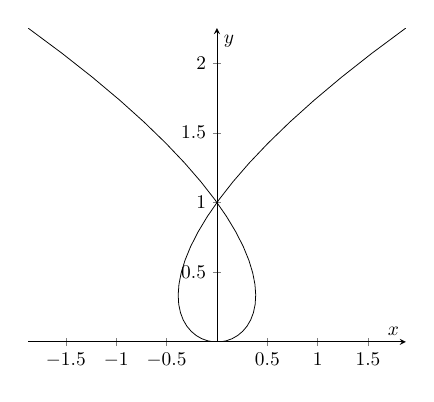
\begin{tikzpicture}[scale=0.7]
\begin{axis}[
    axis lines = middle,
    xlabel = $x$,
    ylabel = $y$,
]
\addplot[
    domain=-1.5:1.5,
    samples=50,
]
({x^3 - x}, {x^2});
\end{axis}
\end{tikzpicture}
  
      \end{center}
      Note que uma imersão pode não ser injetiva globalmente, mas é injetiva localmente.
  \end{itemize}
\end{note}
\begin{example}
  A Cicloide não é uma imersão. $g(t)=(t-\sen(t),1-\cos(t))$.
  \begin{center}
    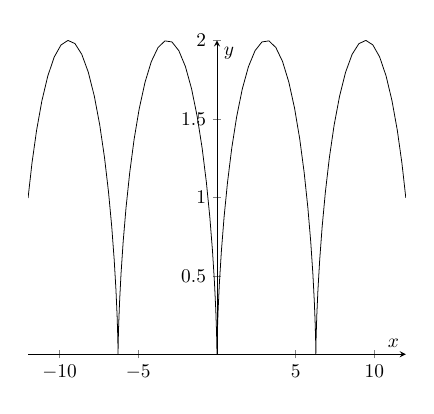
\begin{tikzpicture}[scale=0.7]
\begin{axis}[
    axis lines = middle,
    xlabel = $x$,
    ylabel = $y$,
]
\addplot[
    domain=-11:11,
    samples=100,
]
  ({x - sin(deg(x))}, {1 - cos(deg(x))});
\end{axis}
\end{tikzpicture}
  
  \end{center}
  \begin{itemize}
    \item $g\in C^{\infty}$.
    \item $g$ é injetiva.
    \item $g$ não é imersão, poiss $g^{\prime}(t)=(1-\cos(t),\sen(t))$, logo $g^{\prime}(t)=0$ se, somente se, $t=2k\pi$ com $k\in\mathbb{Z}$. 
  \end{itemize}
\end{example}
\begin{theorem}[Forma local das imersões]
  Seja $U\subseteq \mathbb{R}^{n}$ aberto e $f:U\to\mathbb{R}^{n+m}$ uma aplicação $C^{k}$, $k\geq 1$, tal que $f$ é uma imersão em $a\in U$. Então, existem abertos $A\subseteq U$ com $a\in A$, $W\subseteq \mathbb{R}^{n+m}$, com $f(a)\in W$ e um difeomorfismo $G:W\to G(W)\subseteq\mathbb{R}^{n+m}$ tal que $G\circ f:A\to\mathbb{R}^{n+m}$ satisfaz $(G\circ f)(x)=(x,0)$ para todo $x\in A$. 
\end{theorem}
\begin{proof} 
  \begin{center}
    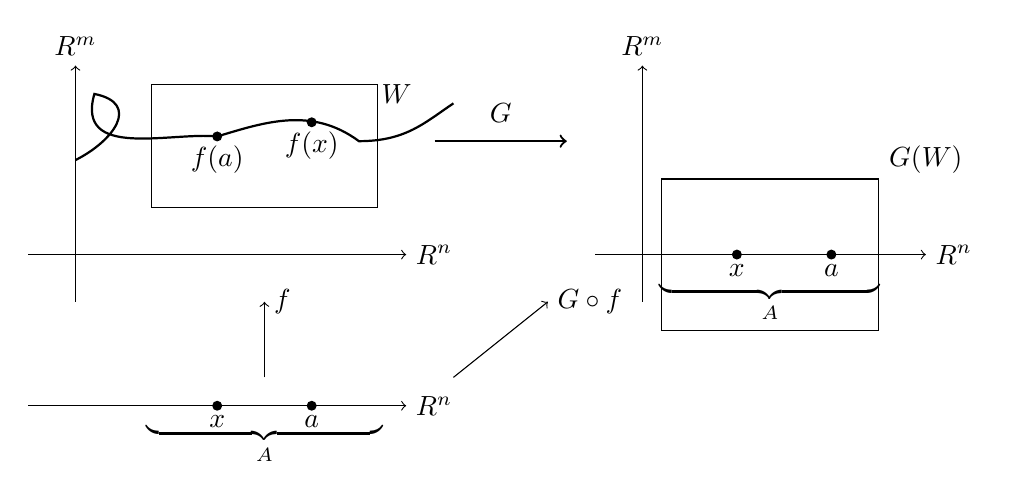
\begin{tikzpicture}[scale=1.2]

  % Ejes izquierda
  \draw[->] (-3,-0.5) -- (-3,2) node[above] {$\mathbb{R}^m$};
  \draw[->] (-3.5,0) -- (0.5,0) node[right] {$\mathbb{R}^n$};

  % Puntos en A
  \fill (-0.5,1.4) circle (1.5pt) node[below] {$f(x)$};
  \fill (-1.5,1.25) circle (1.5pt) node[below] {$f(a)$};
  
  % Rectángulo (W)
  \draw (-2.2,0.5) rectangle (0.2,1.8);
  \node at (0.4,1.7) {$W$};
  
  % Curva dentro
      \draw[thick] 
      (-3,1) 
      .. controls (-2.6,1.2) and (-2.3,1.6) .. (-2.8,1.7)
      .. controls (-3,1) and (-2,1.3) .. (-1.5,1.25)
      .. controls (-1,1.4) and (-0.5,1.57) .. (0,1.2)
      .. controls (0.5,1.2) and (0.7,1.4) .. (1,1.6);
  
  % Flecha F
  \draw[->, thick] (0.8,1.2) to[out=0,in=180] (2.2,1.2);
  \node at (1.5,1.5) {$G$};
  
  % Ejes derecha
  \draw[->] (3,-0.5) -- (3,2) node[above] {$\mathbb{R}^m$};
  \draw[->] (2.5,0) -- (6,0) node[right] {$\mathbb{R}^n$};
  
  
  % Rectángulo G(W)
  \draw (3.2,-0.8) rectangle (5.5,0.8);
  \node at (6,1) {$G(W)$};
  
  % Conjunto A (intervalo)
  \draw (-2,0) -- (0,0);
  \node at (4.35,-0.5) {
      $\underbrace{\hspace{2.8cm}}_{A}$
  };
  
  % Puntos imagen
  \fill (4,0) circle (1.5pt) node[below] {$x$};
  \fill (5,0) circle (1.5pt) node[below] {$a$};
  
  % Flecha hacia abajo (A a c)
  \draw[->] (-1,-1.3) -- (-1,-0.5) node[right] {$f$};
  \draw[->] (1,-1.3) -- (2,-0.5) node[right] {$G\circ f$};
  
  % Línea inferior
  \fill (-1.5,-1.6) circle (1.5pt) node[below] {$x$};
  \fill (-0.5,-1.6) circle (1.5pt) node[below] {$a$};
  \draw[->] (-3.5,-1.6) -- (0.5,-1.6) node[right] {$\mathbb{R}^n$};

  % Conjunto A (intervalo)
  \draw (-2,0) -- (0,0);
  \node at (-1,-2) {
    $\underbrace{\hspace{3cm}}_{A}$
  };

\end{tikzpicture}
 
  \end{center}
  Sem perdida  de generalidade podemos supor que $f^{\prime}(a)(\mathbb{R}^{n})=\mathbb{R}^{n}\times\{0\}$.\\
  De fato, sabemos que $\dim \Img(f^{\prime}(a))=\dim V=n$. Seja $W=V^{\perp}$, i.é, $\dim W=m$. Agora, consideremos uma base ortogonal de $V$ e $W$, i.é, 
  \begin{align*}
    \begin{cases}
      \{v_1,v_2,\cdots,v_n\}, &\text{ base de } V \text{,} \\
      \{w_1,w_2,\cdots,w_m\}, &\text{ base de } W.
    \end{cases}
  \end{align*}
  Defina $T:\mathbb{R}^{n+m}\to\mathbb{R}^{n+m}$ uma tranformação linear dada por $T(v_i)=e_i$ e $T(w_i)=e_{n+i}$ para todo $i$.\\
  Logo $T$ é um isomorfismo linear e $T(V)=\mathbb{R}^{n}\times\{0\}$ e $T(W)=\{0\}\times\mathbb{R}^{m}$.\\
  Logo, considere a função $\tilde{f}=T\circ f:U\to\mathbb{R}^{n+m}$.\\
  Pela regra da cadeia temos que $\tilde{f}^{\prime}=Tf^{\prime}$ que como $f^{\prime}$ é injetiva e $T$ é bijetiva, temos que $\tilde{f}^{\prime}$ ´e injetiva, logo $\Img \tilde{f}^{\prime}(a)=\mathbb{R}^{n}\times \{0\}$.\\
  Se provamos o teorema para $\tilde{f}^{\prime}$, obtemos que $a\in A$, $\tilde{f}(a)\in W$ e um difeomorfismo $\tilde{G}:W\to\tilde{G}(W)$ tal que $(\tilde{G}\circ\tilde{f})(x)=(x,0)$, logo você pode fazer $G=\tilde{G}\circ T$.\\
  Agora, defina $F:U\times \mathbb{R}^{m}\to\mathbb{R}^{n+m}$ como $F(x,y)=f(p_1(x,y))+p_2(x,y)=f(x)+(0,y)$. Onde $p_1$ e $p_2$ são as projeções de $\mathbb{R}^{n+m}$ sobre $\mathbb{R}^{n}\times\{0\}$ e $\{0\}\times\mathbb{R}^{m}$, respectivamente. Agora, calculamos a derivada de $F$ no ponto $(a,0)$
  \begin{align*}
    F^{\prime}(a,0)\cdot(h,k)=f^{\prime}(a)\cdot h+(0,k).
  \end{align*}
  Logo $\Img(F^{\prime}(a,0))=\mathbb{R}^{n+m}$. Assim, $F^{\prime}(a,0)$ é sobrejetiva, logo como ela é linear é injetiva e portanto ela ´e um isomorfismo invertivel.\\
  Pelo teorema da função inversa temos que existem abertos $V\subseteq \mathbb{R}^{n+m}$ com $(a,0)\in V$ e $W\subseteq\mathbb{R}^{n+m}$ com $F(a,0)=f(a)\in W$ taes que $F\big|_{V}:V\to W$ é um difeomorfismo.\\
  Seja $G:\left[ F\big|_{V} \right]^{-1}:W\to V$ e $A=p_1(V)\subseteq U$, logo para todo $x\in A$ temos que $(x,0)\in V$ e portanto
  \begin{align*}
    (G\circ f)(x)=G(f(x))=(G\circ F)(x,0)=(x,0).
  \end{align*}
  Para todo $x\in A$.
\end{proof}
